\color{Melon}
    На основе анализа, произведенного выше, можно утверждать, что процесс развития криптографии последователен в направлении гомоморфного шифрования. Если симметричная криптография рассматривает вопросы конфиденциального хранения информации, то асимметричная криптография рассматривает вопросы конфиденциальной передачи информации, или, говоря по-другому, криптографические протоколы. Вычислительная криптография рассматривает аспект конфиденциальных вычислений, причем это относится как к данным, над которыми производятся вычисления, так и к алгоритму, по которому они производятся. Сама же последовательность развития заключается в том, что  симметричная криптография может быть интегрирована в асимметричную, а та в свою очередь может быть также интегрирована и рассмотрена с точки зрения вычислительной криптографии. Так, например, в криптографических системах асимметричный протокол исследуется для выработки и передачи секретных ключей, основной же канал передачи данных строится на основании симметичного шифра. В то же время как, и в симметричных, так и в ассиметричных системах могут быть обнаружены элементы гомоморфизма.\par
    Соответственно, не каждая система может обладать гомоморфными свойствами, и не каждый примитив из симметричной криптографии может использоваться при построении ассиметричной системы. Описанные отношения представлены на рисунке ниже.\par

    \begin{figure}[ht]
  \centering
  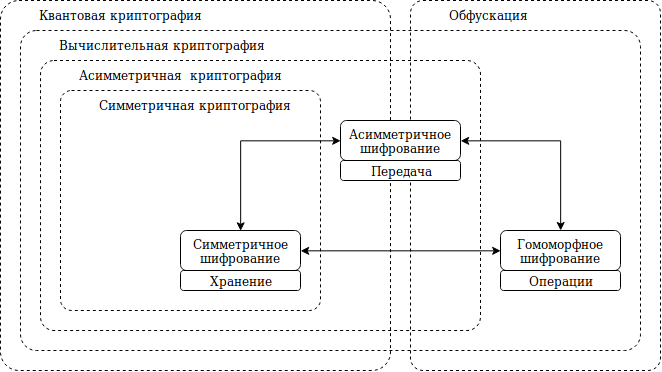
\includegraphics[scale=0.7]{share/struct.png}
  \caption{Криптографическая структура}
  \label{fig:struct}
\end{figure}


    \color{Goldenrod}Также на рисунке обозначены отдельно две области: квантовая криптография и обфускация. Обфускация сама по себе не является частью вычислительной криптографии, однако является производной от нее. В качестве довольно актуального направления, обфускация представляет собой способы обеспечения кофиденциальности, но не пользовательских данных, а самих алгоритмов обработки.\par
    Квантовая же криптография не затрагивает гомоморфное шифрование напрямую, но так как асимметричное или симметричное шифрование может быть частью системы с гомоморнфым шифрованием, то развитие этого направления может оказывать непосредственное влияние.\par
    \color{Plum}Чтобы показать динамику развития, можно отобразить условные элементы, которые представляют собой некоторый уровень абстракции над любой системой шифрования. Для этих элементов выделяются четыре уровня абстракции. Эти уровни затрагиваются в различной мере на различных этапах развития теории шифрования и криптографии, за счет чего и обладают качеством выражения динамических свойств. Этими уровнями являются:  уровень вычислительной проблемы, уровень математических примитивов, уровень криптографических примитивов и уровень криптографической схемы.\par

    \begin{figure}[ht]
  \centering
  
\includegraphics[scale=0.7]{share/el.png}
  \caption{элементы системы гомоморфного шифрования}
  \label{fig:struct}
\end{figure}


    \color{ProcessBlue}Вычислительная проблема характеризует, насколько величина перебора входных данных по значению шифртекста близка по сравнению с граничным значением, представляющим экспоненциальную зависимость от длины шифртекста (значение 2 в степени длины шифртекста). Иными словами, она характеризует качество того, что входные данные нельзя подобрать за время, имеющее полиноминальную зависимость от длины шифртекста.\par
    Набор математических примитивов задаёт множество значений (символов) для шифртекста, его структуру, а также определяет элементарные операции над ним, которые образуют уровень вычислительной проблемы - параметр, связывающий преобразования из открытого текста в шифртекст.\par
    То, какую задачу организует вычислительная проблема посредством математических примтивов, а также функциональное назначение криптосистемы в целом задают криптографические примитивы, например, односторонние функции. Криптографический примитив в системе шифрования определяет, как вычислительная проблема может быть редуцирована, то есть обеспечивает существование неких секретов или ключей.\par
    Наконец, криптографическая схема реализует непосредственно понятие ключа и протокола, то есть модель для конечного использования всей криптосистемы (системы шифрования).\par
    Можно увидеть, что на заре развития теории криптографии, основополагающими уровнем был уровень криптографического примитива, на основе которого изыскивались различные методы шифрования. До асимметричной криптографии никто не мог предположить наличие элементов для криптографической схемы, поэтому можно сказать, что уровни криптографических примитивов и криптографической схемы совпадают, то есть для эры симметричного шифрования не было четкого разделения на уровне вообще, как и понятия системы шифрования.\par
    C появлением асимметричной криптографии появилось наличие публичного/секретного ключа, которым описывается работа криптографической схемы.\color{RoyalBlue}Для этой эры характерно четкое осознание всех уровней, но основные направления исследований сосредоточены на области информационных процессов и протоколов, в которую входят криптографические примитивы и криптографическая схема.\par
    В конце второй эры и начале третьей, внимание ученых сосредоточено на фундаментальных проблемах и, соответственно, на математической области. Можно утверждать в полной мере, что сейчас ученые могут определять и вычислительную область, которая по своей сути обращается на взаимодействие между математическими и криптографическими примитивами. В этом случае, математическая область составляется как бы мощность гомоморфных вычислений, ту ошибку, которая накапливается после каждой операции, а область информационных процессов составляет некий количественный буфер, способность выдерживать эту ошибку. Гомоморфное шифрование имеет непосредсвенную зависимость от математических и криптографических примитивов, отражая таким образом как межуровневую связь, так и связь с различными областями.\par
\normalcolor
